\begin{frame}
   \frametitle{Simulation et analyse statistique des traces des simulations}
   %\framesubtitle{work with Guillaume Taupiac}


\begin{columns}
\begin{column}{0.5\textwidth}

\scalebox{0.9}{
\begin{tikzpicture}[scale = 0.8]
       
    \draw[thick, ->] (-.2,-.1)--(7,-.1) node[below]{$t$};
     \foreach \t in {1,2,3,4,5,6}
      \draw[very thick] (\t,-1pt)--(\t,-2pt) node[below,blue]{\small\t};

     \draw[thick, ->] (0,-.2)--(0,3) node[left]{$Niveau$};
     \foreach \y in {0,1,2}
      \draw[very thick] (2pt,\y)--(-2pt,\y) node[left,blue]{\small\y};
    
    
    \draw[thick,dotted,blue] (0,0) -- (2,0) node[below]{}; 
    \draw[thick,dotted,blue] (2,0) -- (2,1) node[below]{}; 
    \draw[thick,dotted,blue] (2,1) -- (4,1) node[below]{};
    \draw[thick,dotted,blue] (4,1) -- (4,0) node[below]{};
    \draw[thick,dotted,blue] (4,0) -- (6,0) node[below]{};
    \node[instruct,align=center] (mot2) at (4,2) {$\omega=010$};

\end{tikzpicture}
}


%deuxième exemple 
\scalebox{0.9}{
\begin{tikzpicture}[scale = 0.8]
       
    \draw[thick, ->] (-.2,-.1)--(7,-.1) node[below]{$t$};
     \foreach \t in {1,2,3,4,5,6}
      \draw[very thick] (\t,-1pt)--(\t,-2pt) node[below,blue]{\small \t};

     \draw[thick, ->] (0,-.2)--(0,3) node[left]{$Niveau$};
     \foreach \y in {0,1,2}
      \draw[very thick] (2pt,\y)--(-2pt,\y) node[left,blue]{\small \y};
    
    
    \draw[thick,dotted,blue] (0,0) -- (1,0) node[below]{}; 
    \draw[thick,dotted,blue] (1,0) -- (1,1) node[below]{}; 
    \draw[thick,dotted,blue] (1,1) -- (2,1) node[below]{};
    \draw[thick,dotted,blue] (2,1) -- (2,2) node[below]{};
    \draw[thick,dotted,blue] (2,2) -- (3,2) node[below]{};
    \draw[thick,dotted,blue] (3,2) -- (3,1) node[below]{};
    \draw[thick,dotted,blue] (3,1) -- (5,1) node[below]{};
    \draw[thick,dotted,blue] (5,1) -- (5,0) node[below]{};
    \draw[thick,dotted,blue] (5,0) -- (6,0) node[below]{};
    \node[instruct,align=center] (mot2) at (5,2) {$\omega=01210$};
   

\end{tikzpicture}
}


\end{column}


\begin{column}{0.5\textwidth}

Pour chaque composant \tval{$C_{i}$, $1 \leq i \leq P$},
\tval{$N$} simulations génèrent \tval{$\omega_{i1}, \omega_{i2}, \ldots ,\omega_{iN}$} mots.




Pour $1 \leq j \leq N$

%\newline
%\vspace{1cm}



\scalebox{0.9}{
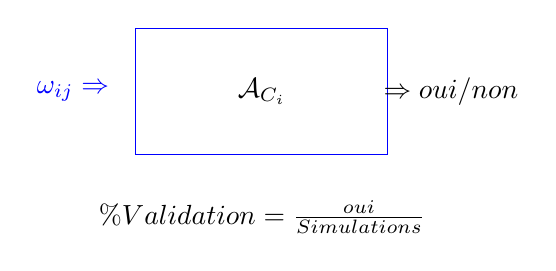
\begin{tikzpicture}[scale = 0.8]
    
    \node[align=center,blue] (mot) at (2,3) {$\omega_{ij} \Rightarrow $};
    
    \draw[blue] (3,2) rectangle (7,4);

    \node[align=center] (automaton) at (5,3) {$\mathcal{A}_{C_{i}}$};
    
    \node[align=center] (accept) at (8,3) {$\Rightarrow \tval{oui}/\alert{non} $};
    
    \node[align=center] (percent) at (5,1) {\tval{$\% Validation = \frac{\card{oui}}{\card{Simulations}}$}};
   

\end{tikzpicture}
}



\end{column}
\end{columns}
\end{frame}